\section{Esercizio 28}
\textit{\textbf{Descrizione:}  Con riferimento alla matrice $A_{N}$ definita in $(1)$,  risolvere il sistema lineare $A_{N}x=(1,\cdots,1)^{T}\in \mathbb{R}^{N}$ con i metodi di Jacobi e Gauss-Seidel, per $N = 10:10:500$, partendo dalla approssimazione nulla della soluzione, ed imponendo la norma del residuo sia minore di $10^{-8}$. Utilizzare, a tale fine, la function dell'esercizio 26, scrivendo function ausiliare $ad hoc$ (vedi esercizio 27) che sfruttino convenientemente la struttura di sparsità (nota) della matrice $A_{N}$.  Graficare il numero delle iterazioni richieste dai due metodi iterativi, rispetto ad $N$, per soddisfare il criterio di arresto prefissato.}
\noindent\emph{Soluzione: }\newline
\lstinputlisting{resources/es28/splitting.m}
\lstinputlisting{resources/es28/matvec.m}
\lstinputlisting{resources/es28/jacobi.m}
\lstinputlisting{resources/es28/gaussSeidel.m}
\lstinputlisting{resources/es28/es28.m}
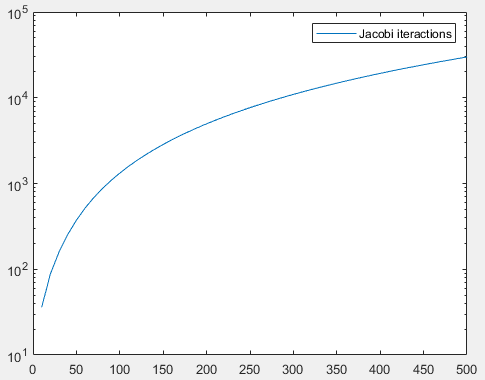
\includegraphics[width=1\linewidth]{img/JacobiIter.png}
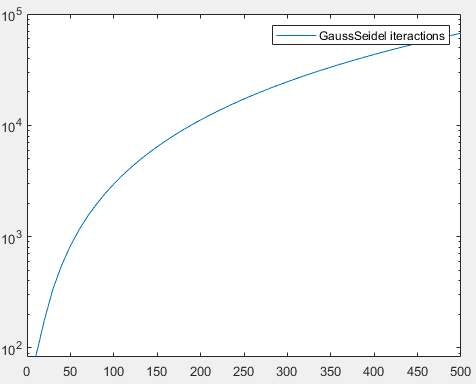
\includegraphics[width=1\linewidth]{img/GSiter.png}
